%\documentclass{article}
%\usepackage{hyperref}
%\usepackage[utf8]{inputenc}
%\usepackage{graphicx}
%\usepackage{booktabs}
%\graphicspath{{schema/}}
%\title{Performance Estimation of the Speed and Distance Monitoring}
%
%\author{Alexander Nitsch \and Benjamin Beichler}
%\date{\today}
%
%\newcommand{\tbi}[1]{$<$\textit{#1}$>$}
%
%% Starts a new line nearly everywhere
%\newcommand{\nl}{\mbox{}\\}
%\newcommand{\nlskip}[1]{\mbox{}\\[#1]}
%
%%
%%Comments
%\newcommand{\cmmnt}[1]{\framebox{#1}}
%\newcommand{\bgcmmnt}[1]{\nl\framebox{\parbox{.95\textwidth}{#1}}\nl[2mm]}
%%\renewcommand{\bgcmmnt}[1]{}
%%
%
%\newcommand{\eod}{\nl\rule{.95\textwidth}{1pt}\nl\textit{End of Document}}
%
%\begin{document}
%\maketitle
%\begin{abstract}
%  This document reports the verification activities of the University of Rostock. SystemC (performance analysis), executable models: SysML modelling and code generation, Scade modeling and code generation.
%\end{abstract}


\mychapter{4}{University of Rostock: Verification of the Speed and Distance
Monitoring}
\label{sec:urostock}
This section reports the verification activities of the \emph{Speed and Distance Monitoring} with model based simulation and virtual prototyping. The first activity pursues the goal of formalizing the specification in the form of an executable model. This model provides a performance estimation at an early stage of system level design and adduces evidence what hardware resources (hardware platform) will be needed for the future OBU. Secondly, finding and reporting of unclarities, inconsistencies, incompleteness and errors while implementing the specification by using tools of the openETCS toolchain (Papyrus/SysML, Scade Suite). Furthermore, we are developing a method of SystemC code generation from abstract and domain specific SysML models. Finally we want to demonstrate the efficiency of model based simulation after transformation from SysML to SystemC models.

The activity is described in the Verification and Validation Plan section {\em 5.3.10 Verification with Model-Based Simulation} \cite{D4.1_2013}. To sum up, we develop application models from the specification of the \emph{Speed and Distance Monitoring}, generate test scenarios and use the inherent simulation environment of SystemC to do performance and scheduling analysis.

\paragraph{Object of verification}  Speed and Distance Monitoring ERTMS function baseline 3.
The system under test is the implemented SystemC code which is described here: \url{https://github.com/openETCS/model-evaluation/tree/master/model/SystemC_TWT_URO/3.13_Speed_and_distance_monitoring}. It describes the Speed and Distance Monitoring at the Software phase.
\nl

\begin{figure}[h]
\centering
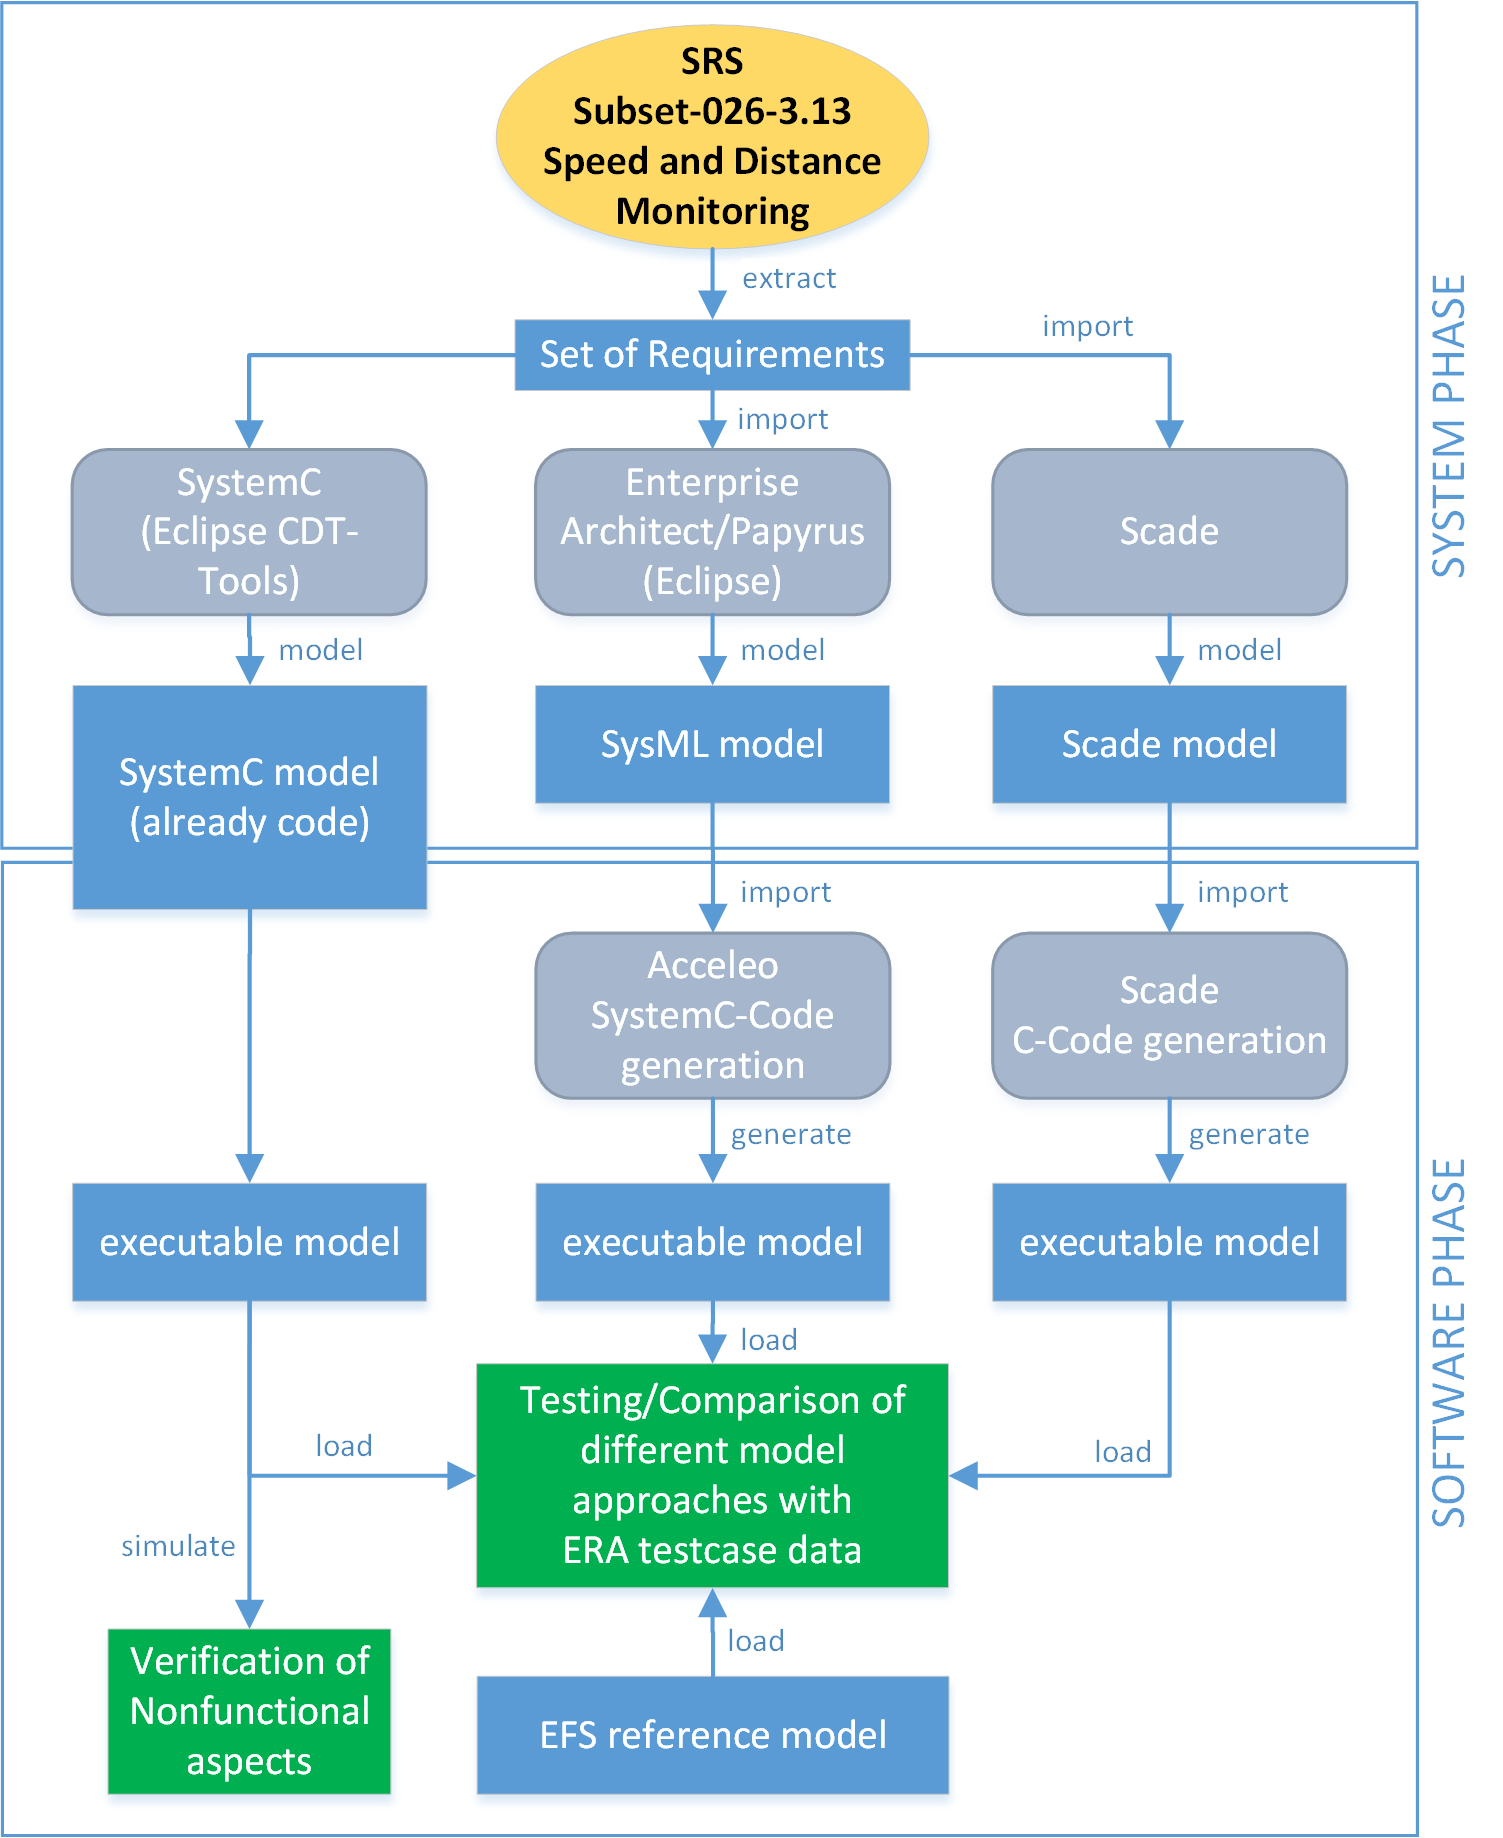
\includegraphics[width=.80\textwidth]{schema/UniRostockApproach.png}
\vspace{4mm}
\caption{University of Rostock VnV Approach}
\label{fig:University of Rostock VnV Approach} 
\end{figure}

\section{Available specification}

The specification is described in the SUBSET-026 Chapter 3.13 \cite{unisig_subset-026_2012}. It describes the realization of both Train Interface (TI) and Driver Machine Interface (DMI) commands by calculating several modules with inputs form train side, track side and odometry. The University of Rostock focuses on the calculation of parts, which are used for safety critical cases using emergency brakes. This especially includes the EBD (emergency brake deceleration) curves.

\section{Detailed verification plan}

\subsection{Goals}

On the one hand we are testing extra-functional aspects such as performance and scheduling analyses to give evidence which hardware system is sufficient to meet the system requirements. We want to discover which hardware resources (e.g. number of processors) will be needed for the OBU. This is important to avoid excessive delays to ensure adequate response times in critical situations. Therefore the University of Rostock will do model based simulation using the inherent simulation environment of SystemC.

On the other hand we use the existing SystemC model to check against a reference model, such as EFS braking curve model. Furthermore we use different tools and means to build additional system models for comparison and verifying behavior.

\subsection{Method/Approach}

Figure \ref{fig:University of Rostock VnV Approach} depicts our methodology. Three models will be created from the specification (SRS): one SystemC model that is directly implemented (hand written) into executable code (finished), one SysML model that will be used to produce (automatically) SystemC code to be executable (not finished) and one Scade Suite model that will be used to produce C code (not finished). For model verification we use test cases and data provided by WP4 and use the ERA excel datasheet as reference implementation. The created test models will contain behavioral representation of the \emph{Speed and Distance Monitoring} such as state machines, activity diagrams and sequence diagrams. There will be a link to the specification requirements to meet the needs of traceability in terms of verification activities.


\subsection{Means}

The Artifacts are produced as follow:
\begin{itemize}
\item SystemC code which is directly implemented (hand written source code).
\item One test model is the generated SystemC model. It's code will be generated/transformed by Acceleo from abstract SysML models designed with Enterprise Architect and/or Papyrus.
\item C code is produced by Scade using Scade Suite.
\item Executable code is compiled with GNU-C-Compiler \texttt{gcc}.
\item Reference model (for now because no other is available) delivered by ERTMS Formal Specs.
\item Testdata and testcases are provided in corporation with ERTMS Formal Specs using the ERA excel data sheet.
\end{itemize}

\subsection{Results}

Verification of extra-functional aspects is successfully done for the first iteration of application models. The provided results consist of recommendations on how hardware resources shall be allocated to the future OBU. The modeling activities are still in progress.

\subsection{Summary}

What we have done:
\begin{enumerate}
\item Created an executable model in SystemC.
\item Ran simulations on single, dual and multi core virtual prototypes.
\item Architecture SysML model of the \emph{Speed and Distance Monitoring}.
\item Architecture Scade model of the \emph{Speed and Distance Monitoring}.
\item Defined a reduced set of parameters for calculating braking Curves especially EBD curves.
\end{enumerate}
 
 The next step:
 \begin{enumerate}
 \item Finishing model activities on SysML and Scade.
 \item Developing a model transformation/code generation from SysML models.
 \item Defining an exchanges interfaces between different model approaches.
 \item Run the tests.
 \end{enumerate}
\subsection{Conclusions/Lessons learned}
From the first results, we see that SysML is a very powerful graphical modeling language but to perform code generation it is necessary to have restrictions to it. We will have a domain specific SysML profile to get reliable results from code generation.  


\section{Future Activities}
Simulink as a modeling tool is in our interest because there is a bridge to Scade. Simulink provides code generation for hardware description languages such as VHDL. That enables new hardware test scenarios.